
\begin{figure}[hbt!]
	\centering%
	\caption{Histogram of Stock Prices}%
	\label{fig:histogram_prices}%
	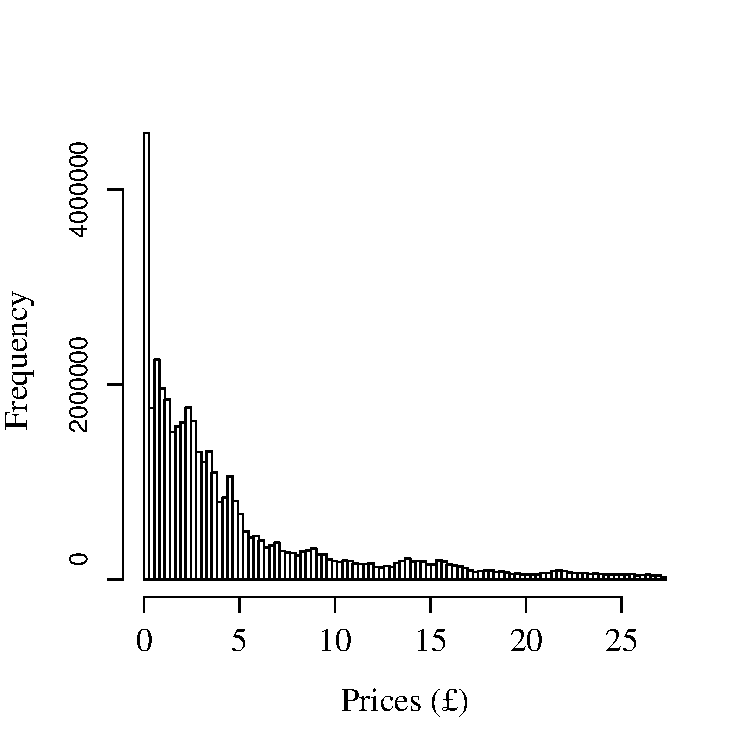
\includegraphics[width=.6\textwidth]{figures/prices_hist_login_days.pdf}
	\fignote{Figure shows the histogram of prices on login days. Outliers above the 95 percentile are excluded.}
\end{figure}

%\clearpage
%
%\begin{figure}[hbt!]
%	\caption{Leftmost Stock Price Digit and Probability of Sale \\ All Login Days}%
%	\label{fig:left_digit_sell_increase_alldays}%
%	\centering%	
%
%		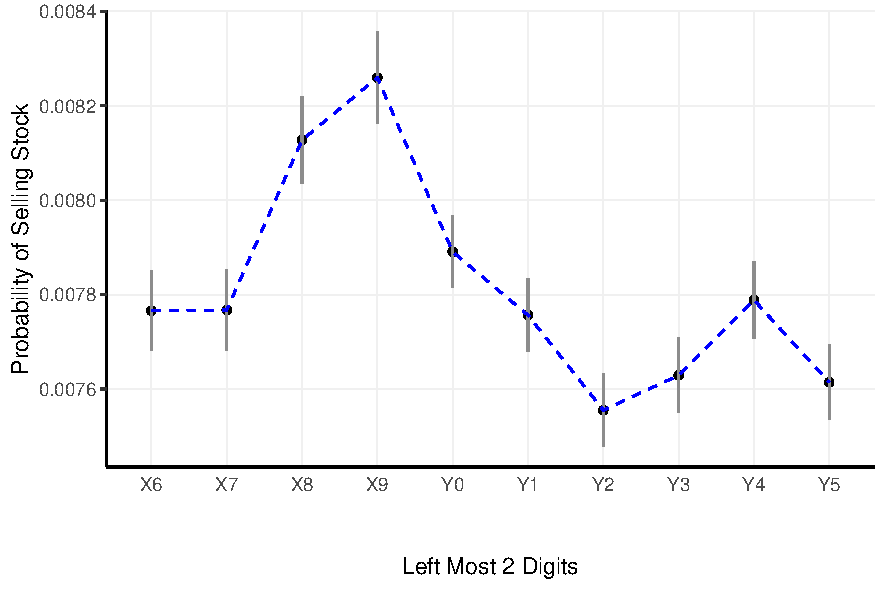
\includegraphics[width=0.6\textwidth]{figures/Left2all_data_probCI.pdf}
%
%	\fignote{£$Y$ in the X-axes is equivalent to £$X+1$ (e.g., £X9 could include £0.19, £1.9, £19, etc., while £Y0 could include £0.20, £2.0, £20, etc.). }
%\end{figure}

\clearpage

\begin{figure}[hbt!]
	\caption{Sample Selection and Simulation Exercise}%
	\label{fig:sample_selection_test}%
	\centering%	
	\bigskip
	\subfigure[Price Increasing Sample]{
%		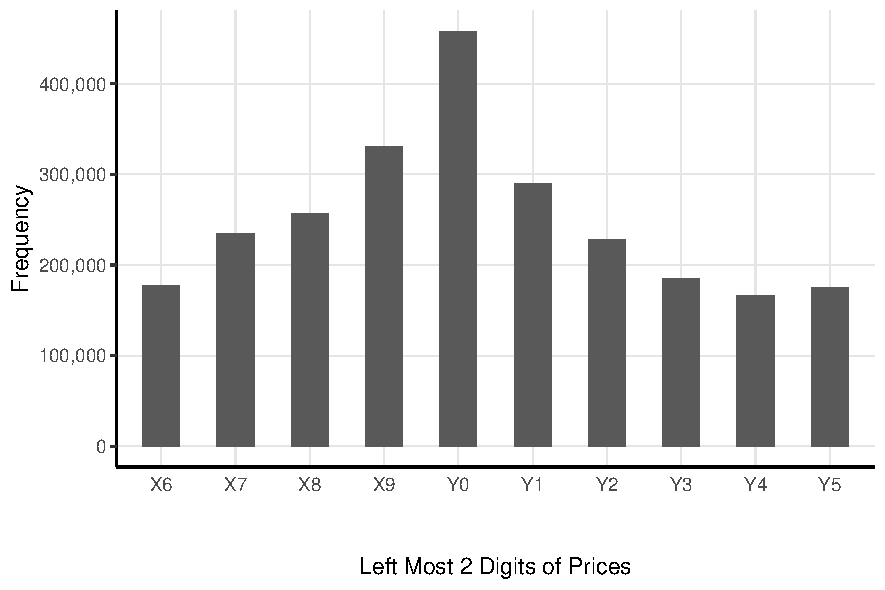
\includegraphics[width=0.45\textwidth]{figures/left2_second_increase_count_quarter.pdf}
		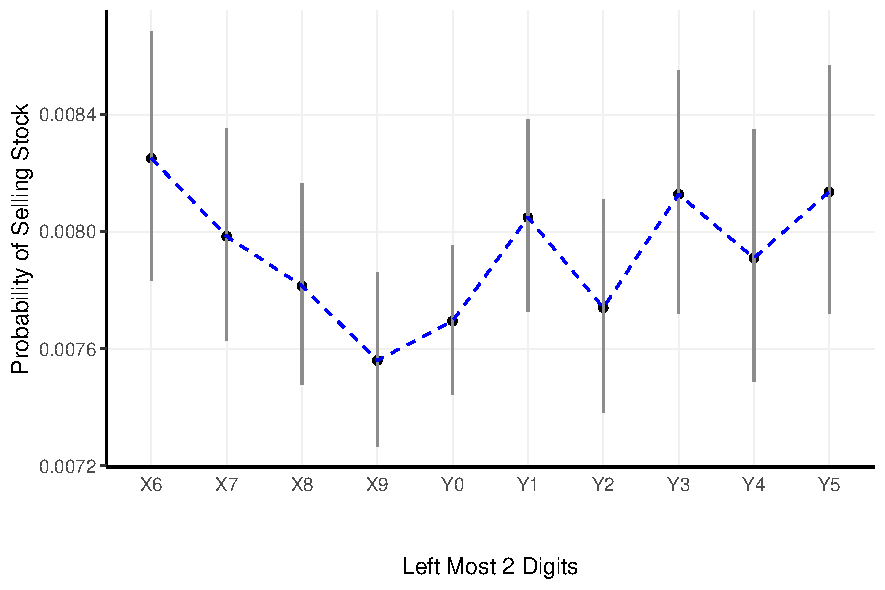
\includegraphics[width=0.45\textwidth]{figures/no_yest_loginLeft2increase_probCI_quarter_random_sell.pdf}
	}
	\subfigure[Price Decreasing Sample]{
%		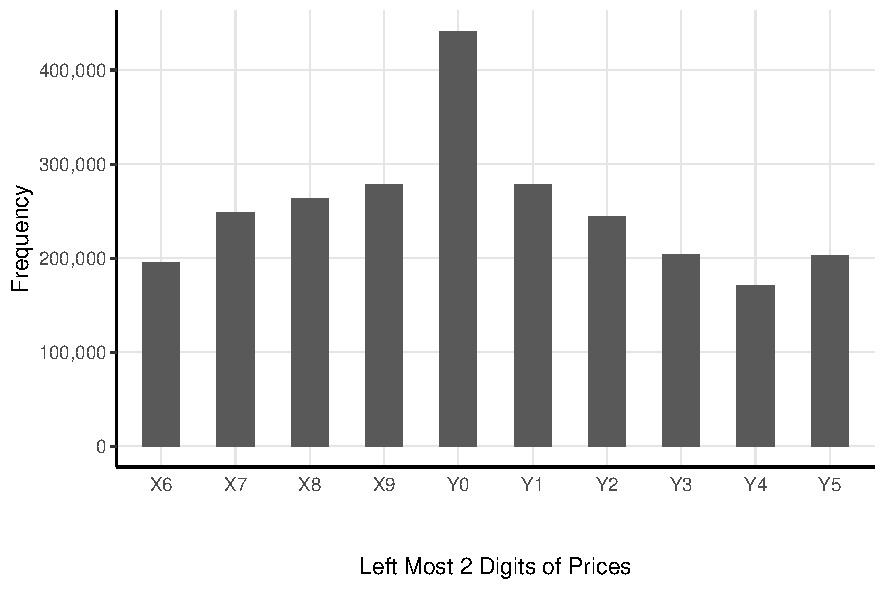
\includegraphics[width=0.45\textwidth]{figures/left2_second_decrease_count_quarter.pdf}
		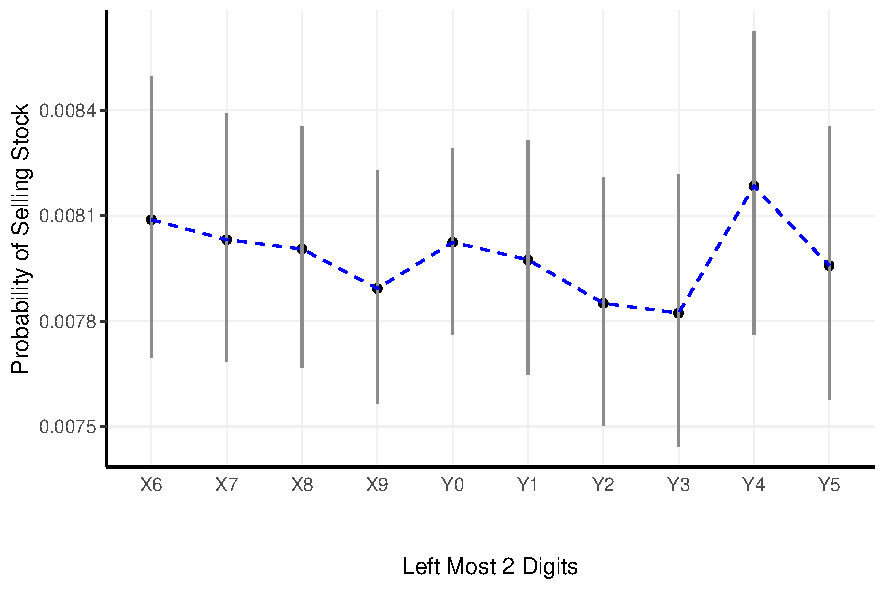
\includegraphics[width=0.45\textwidth]{figures/no_yest_loginLeft2decrease_probCI_quarter_random_sell.pdf}
	}
\end{figure}

\clearpage

\begin{figure}[hbt!]
	\caption{Leftmost Stock Price Digit and Probability of Sale, Monthly Sample}%
	\label{fig:left_digit_sell_monthly}%
	\centering%	
	\bigskip
	\subfigure[Price Increasing]{
		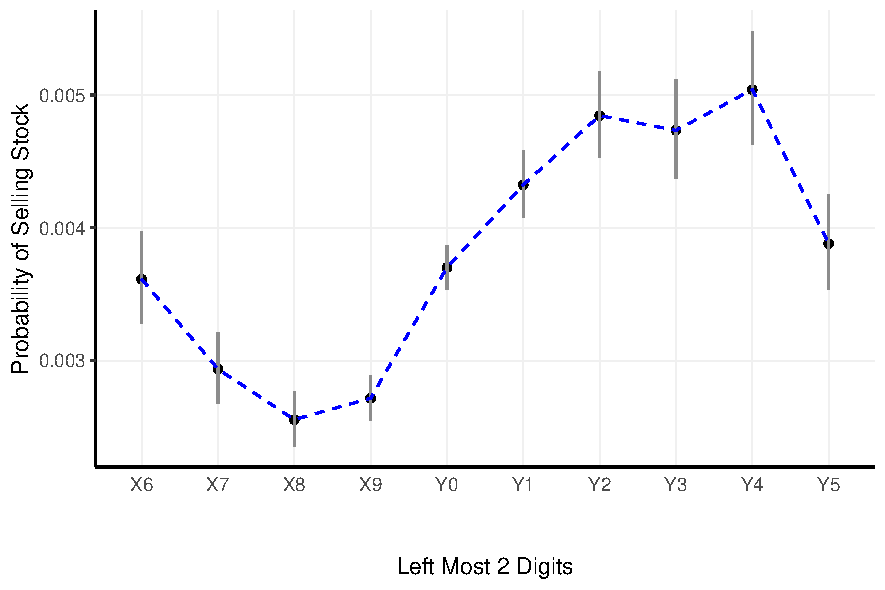
\includegraphics[width=0.45\textwidth]{figures/no_yest_loginLeft2increase_probCI_month.pdf}
		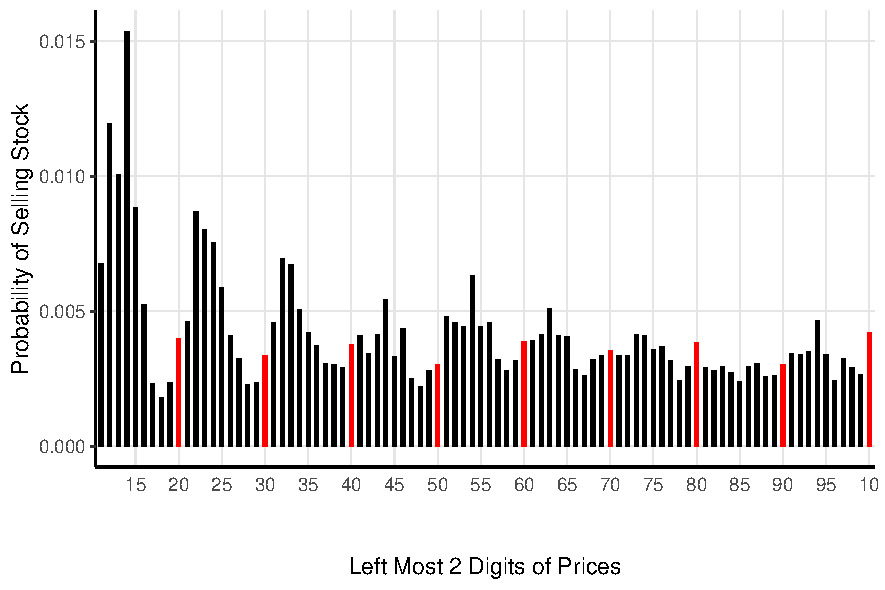
\includegraphics[width=0.45\textwidth]{figures/no_yest_login2left_increase_month.pdf}	
	}
	\subfigure[Price Decreasing]{
		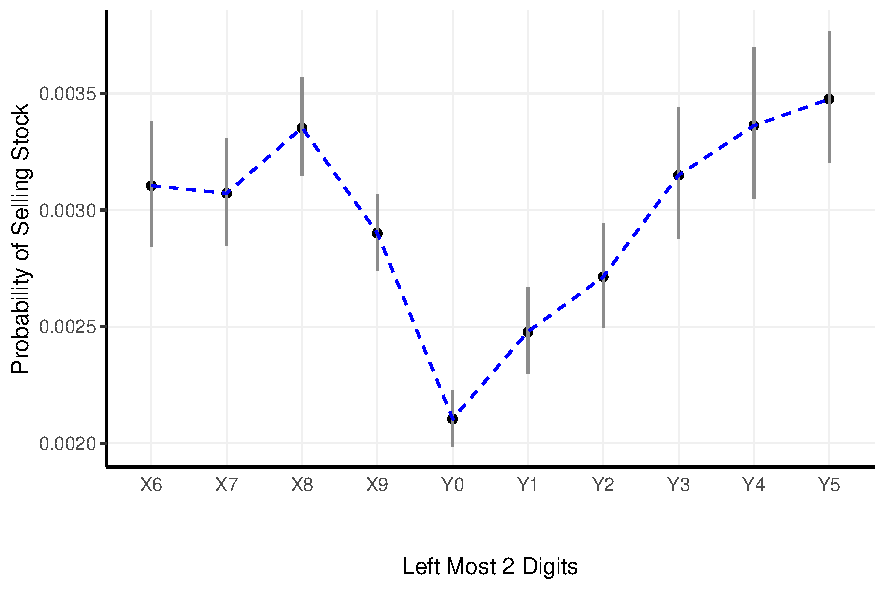
\includegraphics[width=0.45\textwidth]{figures/no_yest_loginLeft2decrease_probCI_month.pdf}
		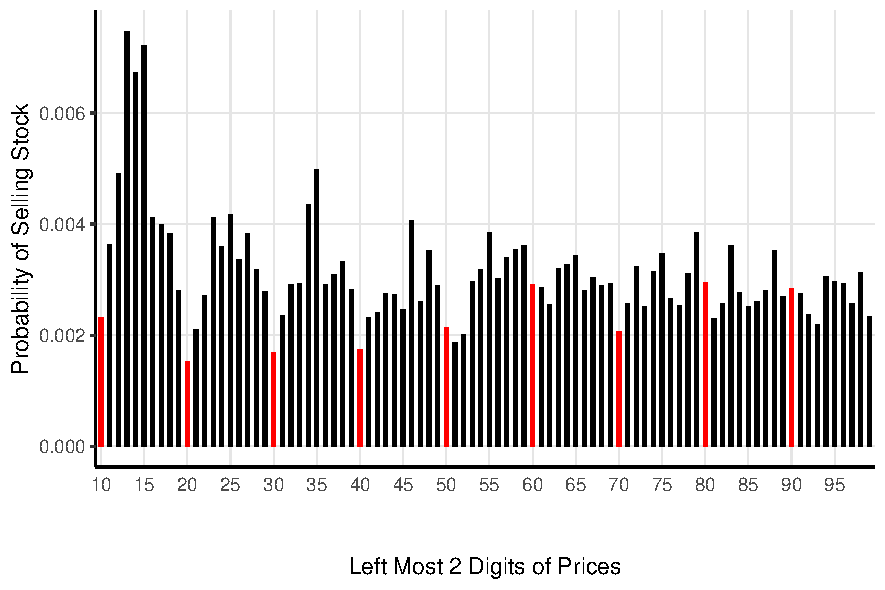
\includegraphics[width=0.45\textwidth]{figures/no_yest_login2left_decrease_month.pdf}	
	}
	\fignote{£$Y$ in the X-axes is equivalent to £$X+1$ (e.g., £X9 could include £0.19, £1.9, £19, etc., while £Y0 could include £0.20, £2.0, £20, etc.).}
\end{figure}

\clearpage

\begin{figure}[hbt!]
	\caption{Leftmost Stock Price Digit and Probability of Sale, Annual Sample}%
	\label{fig:left_digit_sell_annual}%
	\centering%	
	\bigskip
	\subfigure[Price Increasing]{
		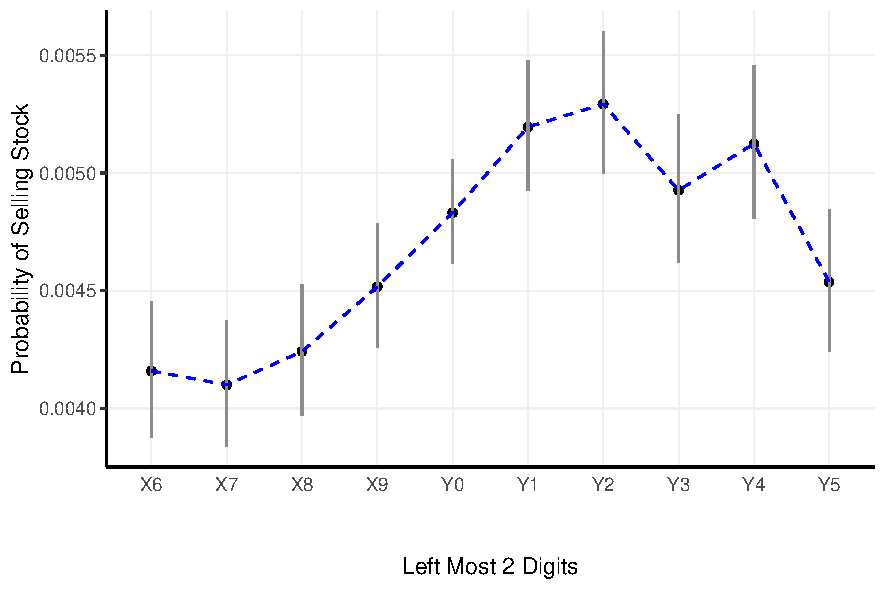
\includegraphics[width=0.45\textwidth]{figures/no_yest_loginLeft2increase_probCI_year.pdf}
		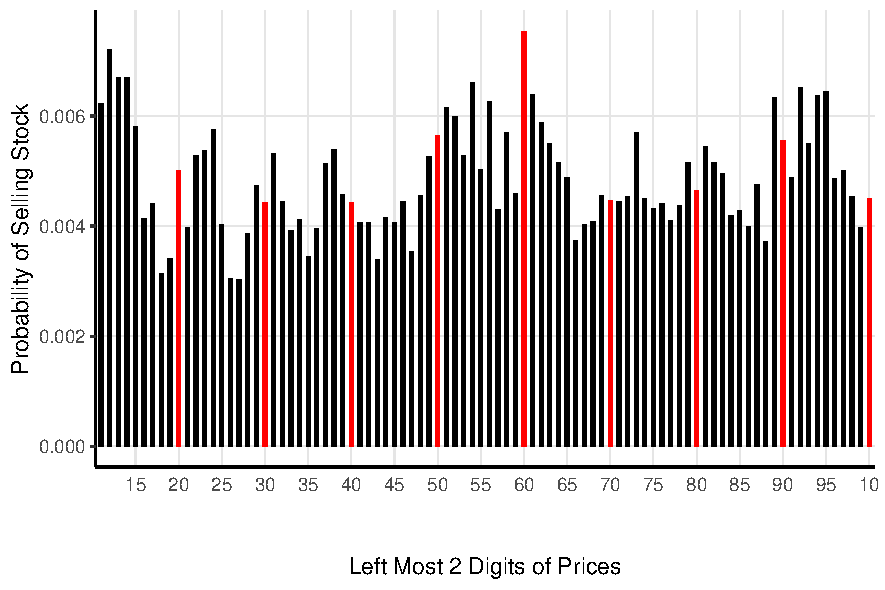
\includegraphics[width=0.45\textwidth]{figures/no_yest_login2left_increase_year.pdf}	
	}
	\subfigure[Price Decreasing]{
		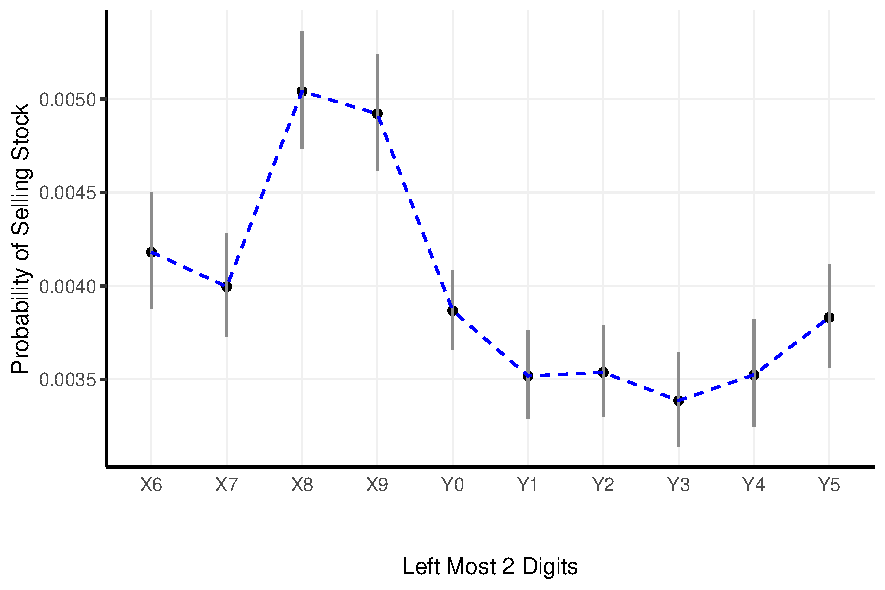
\includegraphics[width=0.45\textwidth]{figures/no_yest_loginLeft2decrease_probCI_year.pdf}
		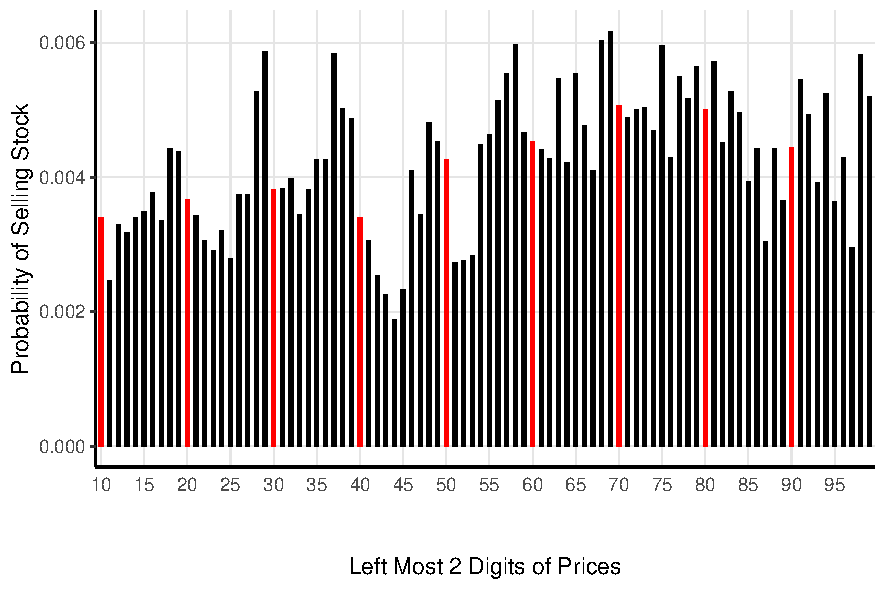
\includegraphics[width=0.45\textwidth]{figures/no_yest_login2left_decrease_year.pdf}	
	}
	\fignote{£$Y$ in the X-axes is equivalent to £$X+1$ (e.g., £X9 could include £0.19, £1.9, £19, etc., while £Y0 could include £0.20, £2.0, £20, etc.).}
\end{figure}

\clearpage

\begin{figure}[hbt!]
	\caption{Leftmost Stock Price Digit and Probability of Sale, Sell Days}%
	\label{fig:left_digit_sell}%
	\centering%	
	\bigskip
	\subfigure[Price Increasing]{
		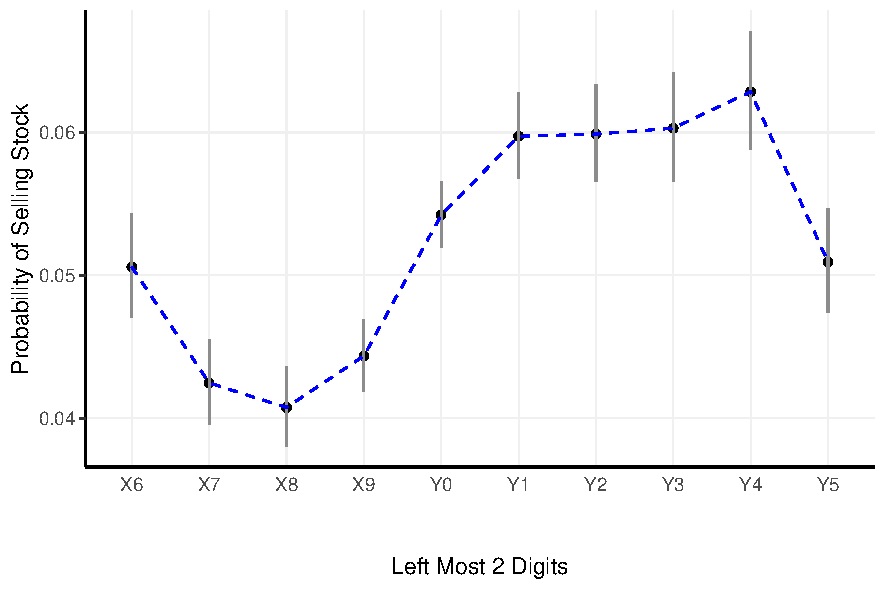
\includegraphics[width=0.45\textwidth]{figures/no_yest_loginLeft2increase_probCI_quarter_sell.pdf}
		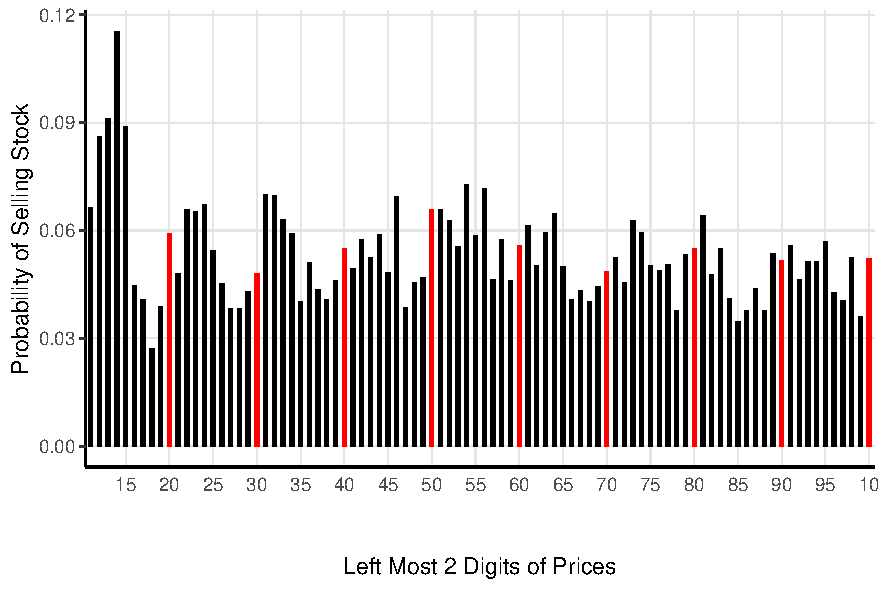
\includegraphics[width=0.45\textwidth]{figures/no_yest_login2left_increase_quarter_sell.pdf}	
	}
	\subfigure[Price Decreasing]{
		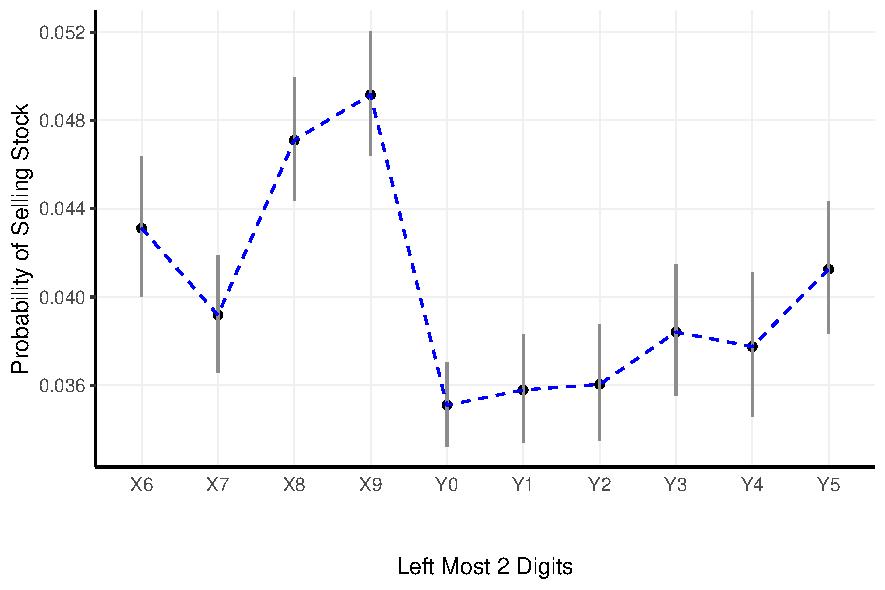
\includegraphics[width=0.45\textwidth]{figures/no_yest_loginLeft2decrease_probCI_quarter_sell.pdf}
		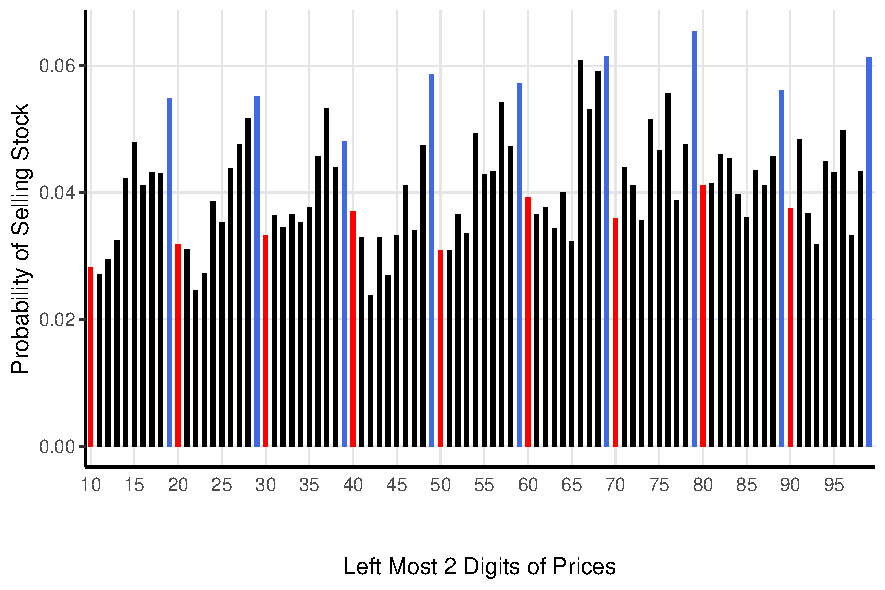
\includegraphics[width=0.45\textwidth]{figures/no_yest_login2left_decrease_quarter_sell.pdf}	
	}
	\fignote{£$Y$ in the X-axes is equivalent to £$X+1$ (e.g., £X9 could include £0.19, £1.9, £19, etc., while £Y0 could include £0.20, £2.0, £20, etc.).}
\end{figure}

\clearpage

\begin{figure}[hbt!]
	\caption{Leftmost Stock Price Digit and Probability of Sale, Sell Days \\ Prices Increasing Sample by Price Range}%
	\label{fig:left_digit_sell_increase_sellsample}%
	\centering%	
	\bigskip
	\subfigure[Price = \pounds0.11 to \pounds1.01]{
		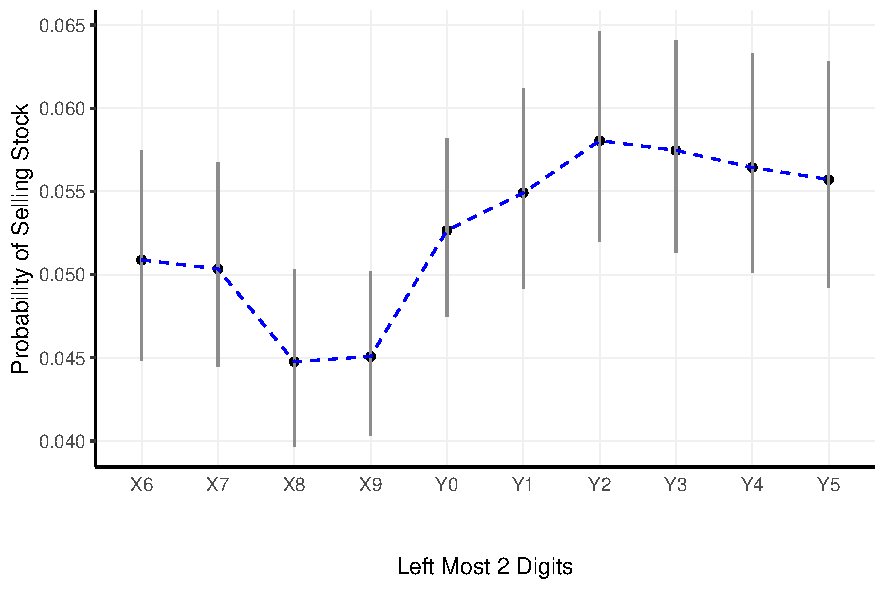
\includegraphics[width=0.45\textwidth]{figures/no_yest_loginLeft2increases_1pbin_CI_quarter_sell.pdf}
		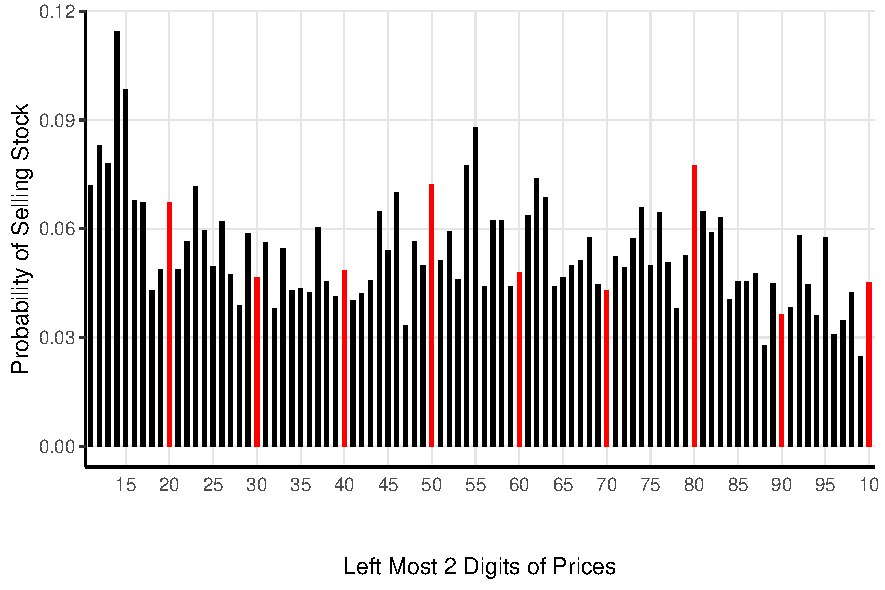
\includegraphics[width=0.45\textwidth]{figures/no_yest_login2left_increase_bin1p_quarter_sell.pdf}
	}
	\subfigure[Price = \pounds1.01 to \pounds10.1]{
		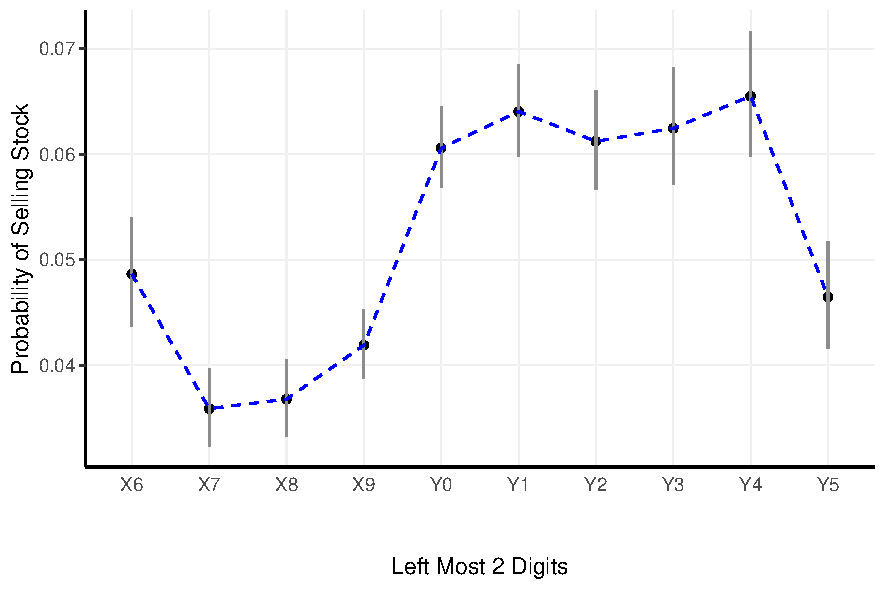
\includegraphics[width=0.45\textwidth]{figures/no_yest_loginLeft2increases_10pbin_CI_quarter_sell.pdf}
		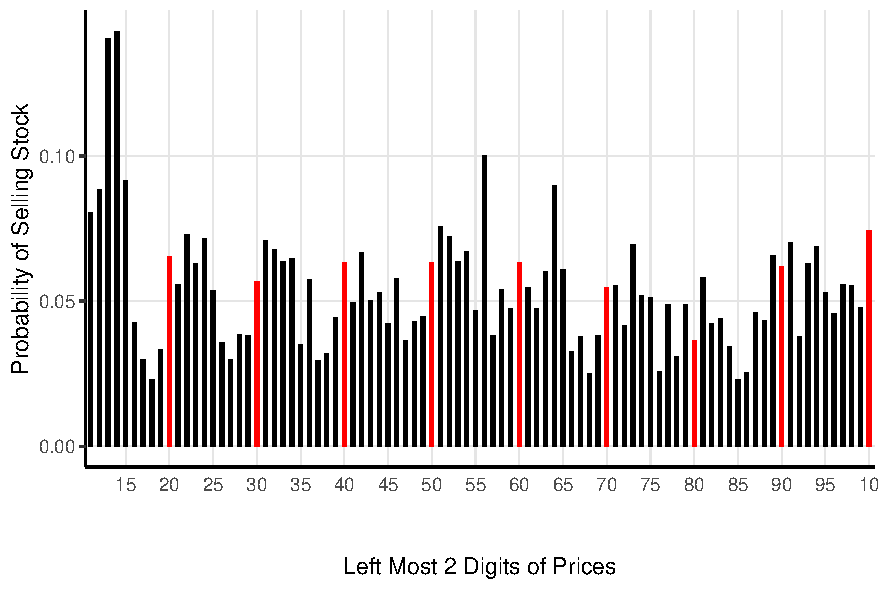
\includegraphics[width=0.45\textwidth]{figures/no_yest_login2left_increase_bin10p_quarter_sell.pdf}
	}
	\subfigure[Price = \pounds11 to \pounds101]{
		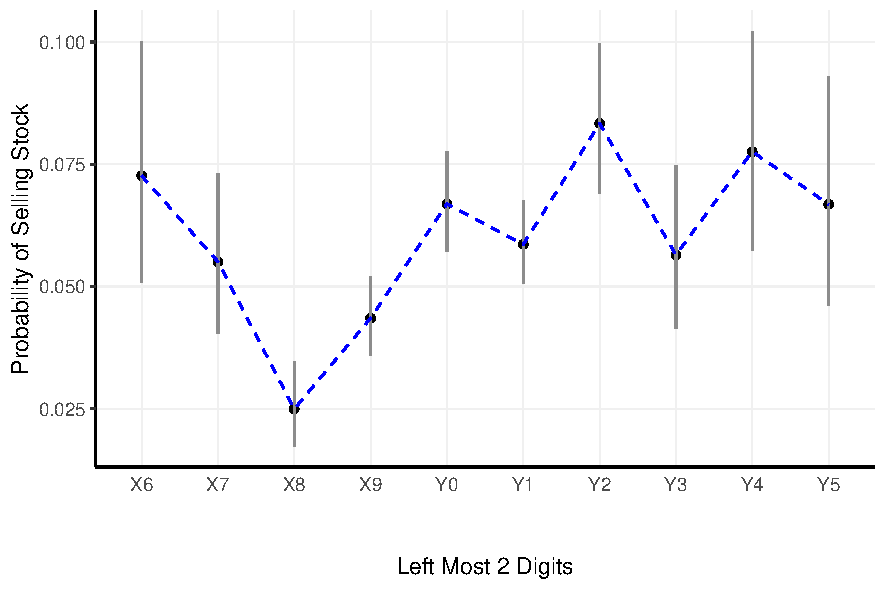
\includegraphics[width=0.45\textwidth]{figures/no_yest_loginLeft2increases_1poundbin_CI_quarter_sell.pdf}
		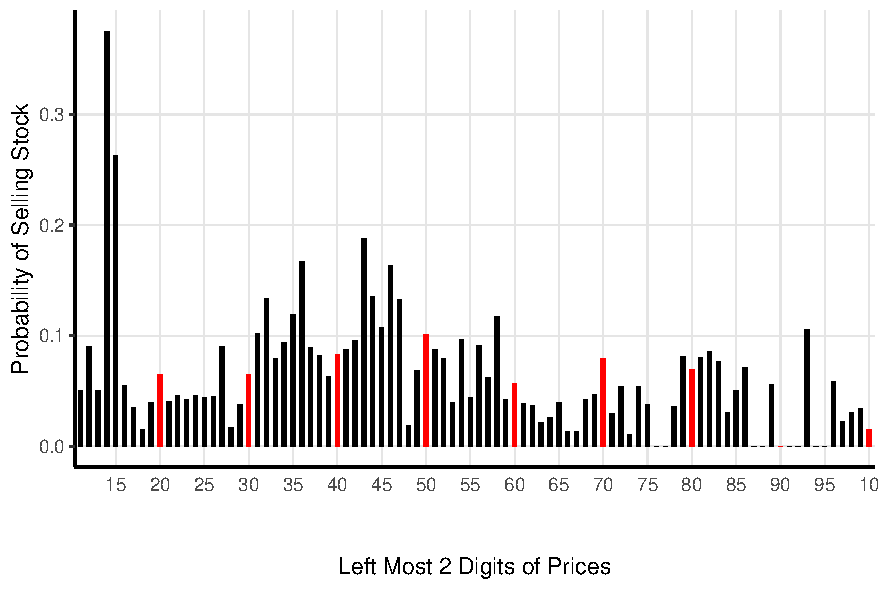
\includegraphics[width=0.45\textwidth]{figures/no_yest_login2left_increase_bin1pound_quarter_sell.pdf}
	}
	\fignote{£$Y$ in the X-axes is equivalent to £$X+1$ (e.g., £X9 could include £0.19, £1.9, £19, etc., while £Y0 could include £0.20, £2.0, £20, etc.). Panels A, B and C show equal size bins of 1p, 10p and £1, respectively. }
\end{figure}

\clearpage

\begin{figure}[hbt!]
	\caption{Leftmost Stock Price Digit and Probability of Sale, Sell Days \\ Prices Decreasing Sample by Price Range}%
	\label{fig:left_digit_sell_decrease_sellsample}%
	\centering%	
	\bigskip
	\subfigure[Price = \pounds0.10 to \pounds1.00]{
		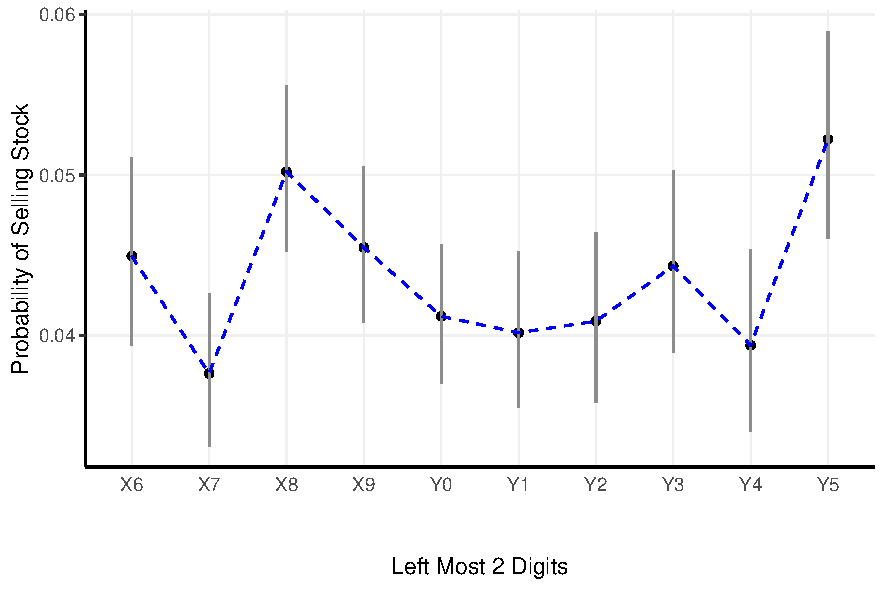
\includegraphics[width=0.45\textwidth]{figures/no_yest_loginLeft2decreases_1pbin_CI_quarter_sell.pdf}
		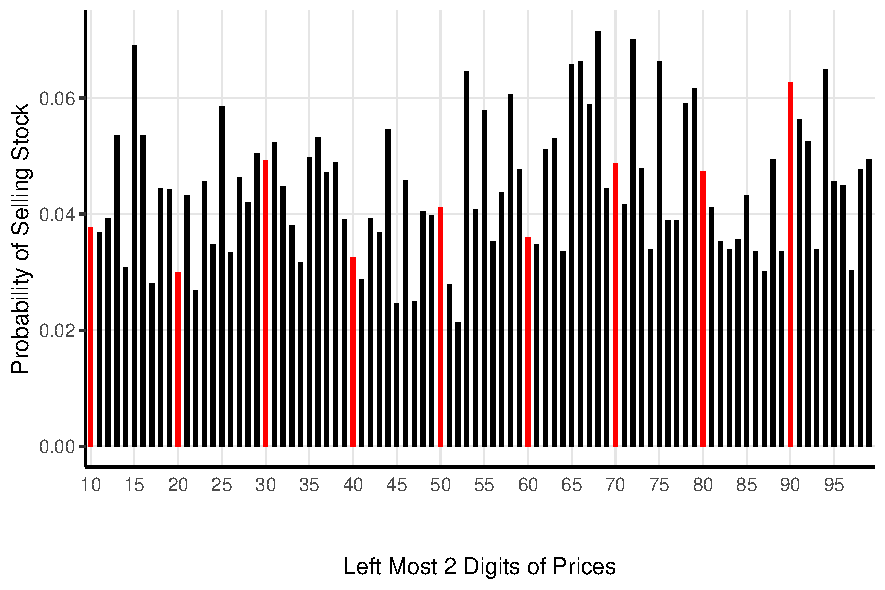
\includegraphics[width=0.45\textwidth]{figures/no_yest_login2left_decrease_bin1p_quarter_sell.pdf}
	}
	\subfigure[Price = \pounds1.00 to \pounds10.0]{
		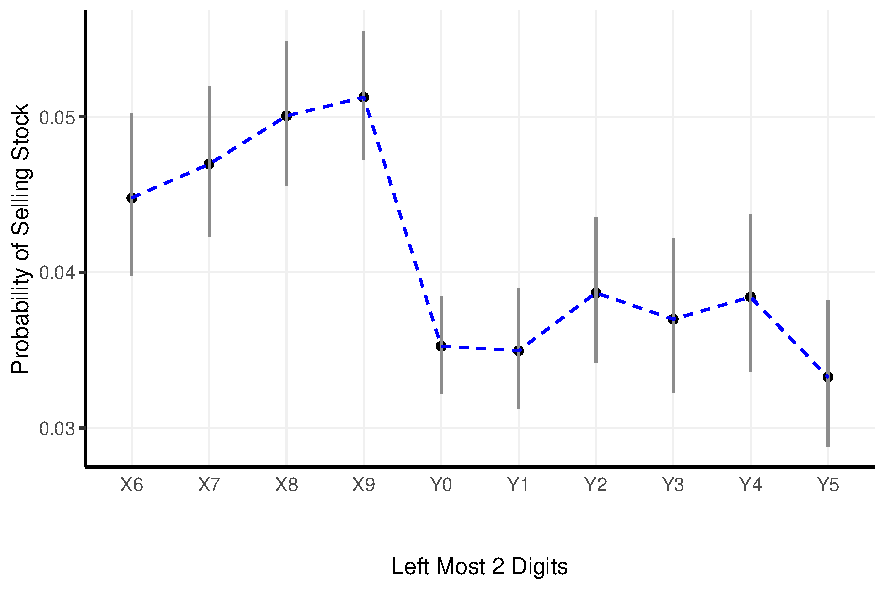
\includegraphics[width=0.45\textwidth]{figures/no_yest_loginLeft2decreases_10pbin_CI_quarter_sell.pdf}
		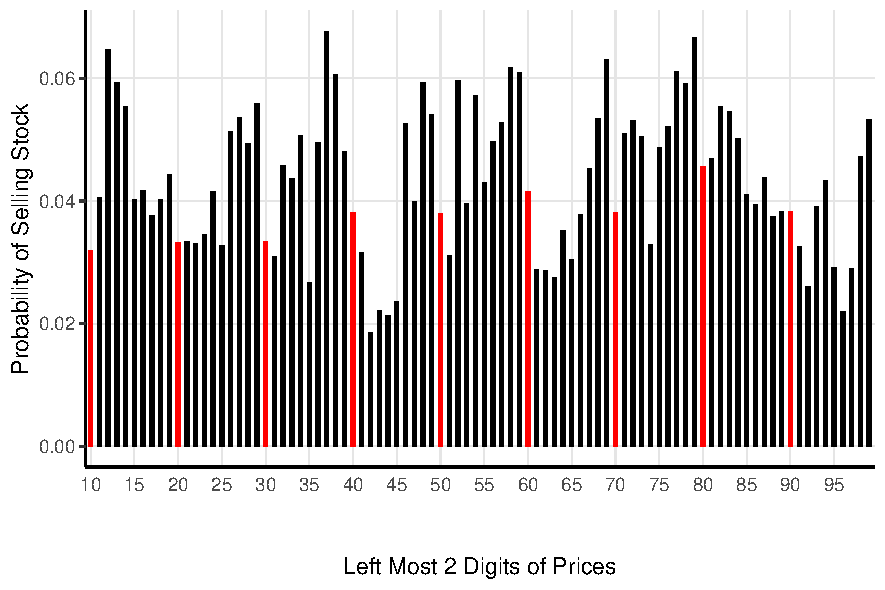
\includegraphics[width=0.45\textwidth]{figures/no_yest_login2left_decrease_bin10p_quarter_sell.pdf}
	}
	\subfigure[Price = \pounds10 to \pounds100]{
		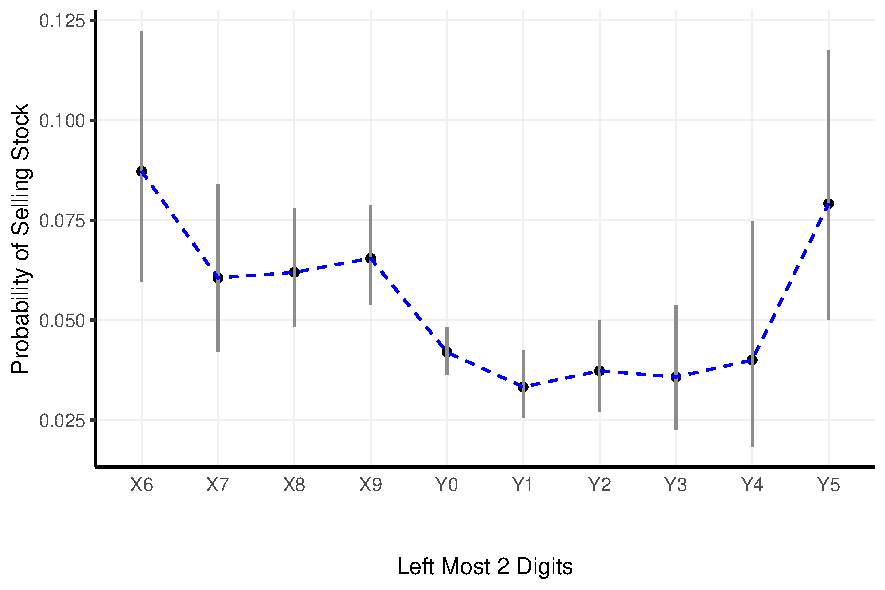
\includegraphics[width=0.45\textwidth]{figures/no_yest_loginLeft2decreases_1poundbin_CI_quarter_sell.pdf}
		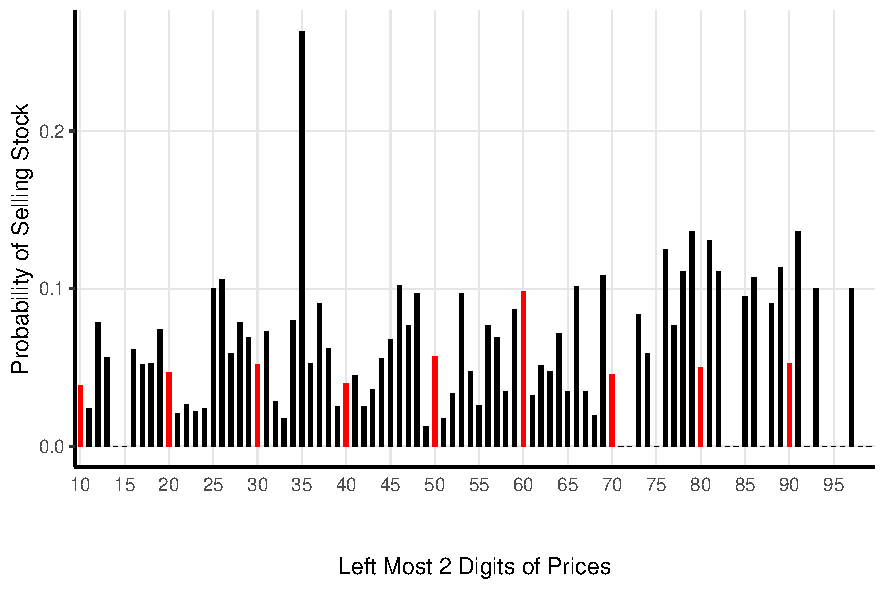
\includegraphics[width=0.45\textwidth]{figures/no_yest_login2left_decrease_bin1pound_quarter_sell.pdf}
	}
	\fignote{£$Y$ in the X-axes is equivalent to £$X+1$ (e.g., £X9 could include £0.19, £1.9, £19, etc., while £Y0 could include £0.20, £2.0, £20, etc.). Panels A, B and C show equal size bins of 1p, 10p and £1, respectively. }
\end{figure}



